\section{Position Bandwidth}

The goal of this test is to find the maximum frequency with which the end-effector can follow a sine trajectory for a specific controller. In order to evaluate this, we create a \emph{Bode-Plot} with the position setpoint as input and the measured position (of the end-effector) as output. The position bandwidth is defined as the frequency with which the amplitude of the output position is reduced by 3dB compared to the amplitude of the setpoint signal.

\subsection{Implementation}

We want to measure a sine wave of different frequencies. At the moment, there has to be a separate measurement for each frequency. In the program, one can set the amplitude, the frequency as well as the number of cycles one wants. For my tests I took 5° as amplitude.

In general, one should use one version of the controller gains for all frequencies, since the bode plot strongly relies on the controller. For my measurements I tried to use the standard sine-params, which worked fine for MIKE \#6 but not for MIKE \#3 (more info in results section).

\subsection{Data Analysis}

The data analysis is more difficult than in other cases. The basic working principle is the following: For each frequency, there is one separate measurement from which the magnitude as well as the phase can be determined. In order to do so, the measured position signal is filtered with a butterworth filter. Afterwards the peaks and their time points of the measured signal as well as the setpoint are extracted. The magnitude can then be calculated by dividing the measured peaks through the setpoint peaks. The phase can be determined from the time points according to the following formula:

\begin{equation}
    \Delta\phi = f*\Delta t*360^\circ
\end{equation}

with
\begin{tabular}{l l}
    $\Delta\phi$ & phase [°]\\
    f & frequency [Hz]\\
    $\Delta t$ & time-difference between setpoint peak and measured peak [s]
\end{tabular}
\vspace{4mm}

However, there are several problems which can occur while reading out the peaks. The most important points which I observed and how I solved them is listed below:

\begin{enumerate}
    \item In the measured signal not all measured peaks represent the amplitude, but can also occur due to control issues or measurement errors.
    
    \emph{solution}: When reading the peaks, I set a certain minimal distance in time between two peaks ($\frac{1}{3*f}$). If the distance between two peaks is smaller, they are neglected.
    
    \item Once I have observed that all the measured minimal-peaks of the setpoint signal are around 0
    
    \emph{solution}: I set the minimal peak-height of the setpoint signal to be 4, this means peaks smaller than 4 are neglected.
    
    \item In the beginning of the trajectory following there is an overshoot for $f>0.2$, resulting in the first measured peak being way too high
    
    \emph{solution}: deleting the first peak measurement for frequencies larger than 0.2
    
    \item All measurements in which the setpoint is 0 are neglected. For $f\geq4$, the last setpoint peak is therefore not reached in the measured signal due to phase shift.
    
    \emph{solution}: delete the last minimal setpoint peak
    
    \item For higher frequencies ($f\geq8$) the system need some time to reach a transient swinging state and the first peak measurements are not reliable.
    
    \emph{solution}: For these frequencies, only the last 20 peaks are used.
    
    \item The minimal and maximal peaks are stored in separate variables. For lower frequencies I have observed that in the measured peaks minimal peaks can be in the maximal peaks and vice versa.
    
    \emph{solution}: All maximal peaks smaller than zero and all minimal peaks larger than 0 are deleted.
    
    \item I have observed that sometimes a peak is measured before the setpoint peak is reached. This can result in more measured peaks than setpoint peaks and a positive phase (impossible).
    
    \emph{solution}: If a measured peak has an earlier time point than the associated setpoint peak, it is deleted.
    
    \item At last I have observed that the phase can increase again for higher frequencies (which is not possible) but can happen due to measurement errors or an insufficient control performance.
    
    \emph{solution}: Before plotting, if a phase of a frequency is closer to zero than the phase of the frequency measured before, it is set to the same phase as measured before (only for $f\geq10$)
\end{enumerate}

\subsection{Results}

The results are presented in the following. It is important to mention here is that the position bandwidth depends mostly on the controller and the chosen gains. Therefore the interpretation of the results is dependant of the goal one wants to examine. If one wants to investigate the performance of one specific controller, it is sufficient to run the test with this controller and to calculate the bandwidth. One could also look for the highest possible bandwidth by comparing different controllers (different sets of controller gains).

I investigated only the performance with the controller gains defined for the sine-params during the initial tuning of the ETH MIKE's. For MIKE \#6 I could use the standard PID-gains and calculated a bandwidth of 6 Hz. For MIKE \#3 I had to change the params a little, as I was not able to run the test stably using the standard sine-params\footnote{The sine params of MIKE \#3 were adjusted after this experiment}. The resulting bandwidth was 10.5 Hz. Compared to Monika's ICORR paper (result: 12Hz), MIKE \#6 is far away. However, then only a PD controller was used and not the real controller running on the MIKE. Maybe one could also improve the bandwidth of the other MIKE versions by a PD controller.

The resulting bode plots are displayed in the following:

\begin{figure}[h]
    \centering
    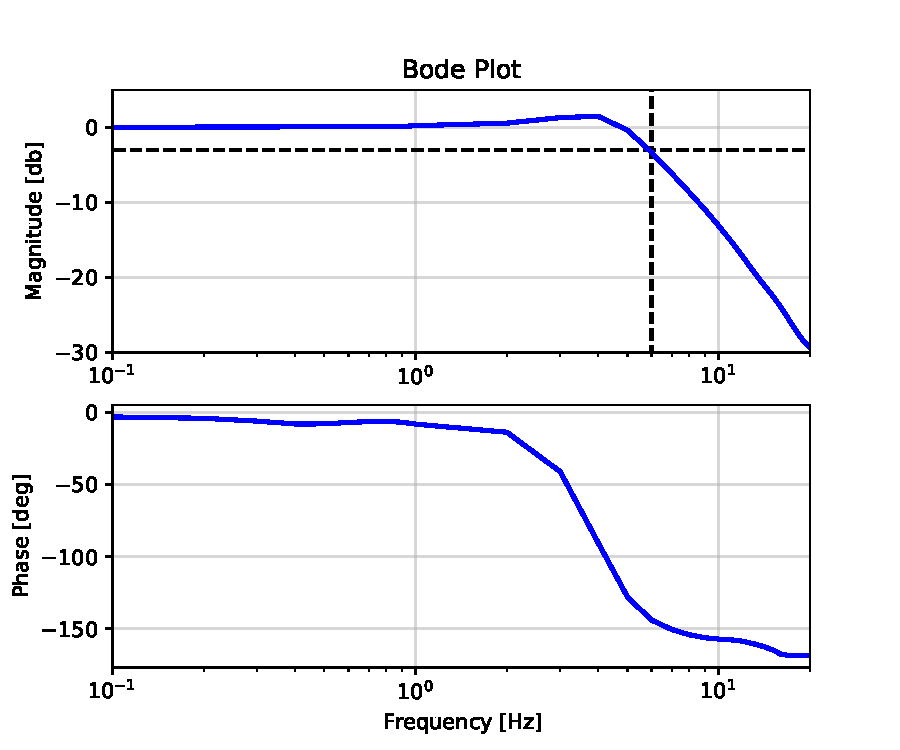
\includegraphics[width = \textwidth]{chapters/position_bandwidth/Mike6_Bode_Plot.pdf}
    \caption{MIKE \#6; Kp=1.2; Ki=6; Kd=0.008; Resulting Bandwitdh=6Hz}
    \label{fig:my_label}
\end{figure}

\begin{figure}[h]
    \centering
    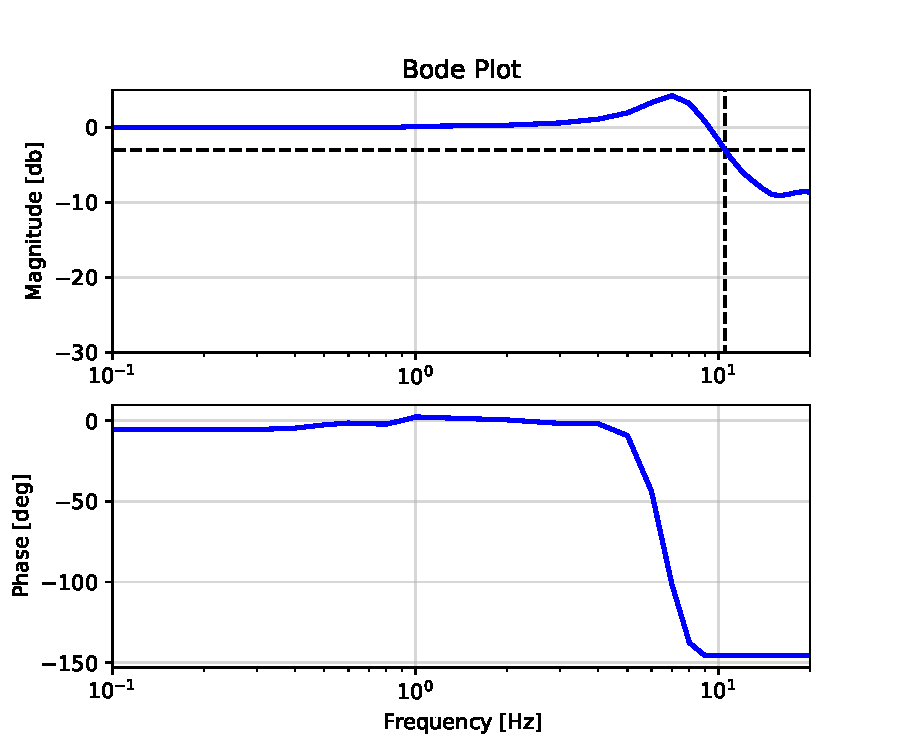
\includegraphics[width = \textwidth]{chapters/position_bandwidth/Mike3_Bode_Plot.pdf}
    \caption{MIKE \#3; Kp=0.5; Ki=5; Kd=0.0006; Resulting Bandwitdh=10.5Hz}
    \label{fig:my_label}
\end{figure}